\documentclass[aspectratio=169,11pt]{beamer}
\usepackage[utf8]{inputenc}
\usepackage[T1]{fontenc}
\usepackage{graphicx}
\usepackage{booktabs}
\usepackage[table]{xcolor}
\usepackage{amsmath}
\usepackage{amssymb}
\usepackage{tikz}
\usetikzlibrary{arrows.meta,positioning,shapes.geometric}

%% ---- Couleurs INPT ----
\definecolor{inptblue}{RGB}{10,48,100}
\definecolor{inptcyan}{RGB}{0,165,215}
\definecolor{inptlight}{RGB}{232,246,252}
\definecolor{myred}{RGB}{180,0,0}

%% ---- Theme ----
\usetheme{Madrid}
\setbeamercolor{structure}{fg=inptblue}
\setbeamercolor{frametitle}{bg=inptblue,fg=white}
\setbeamercolor{block title}{bg=inptblue,fg=white}
\setbeamercolor{block body}{bg=inptlight}
\setbeamercolor{alerted text}{fg=myred}
\setbeamercolor{block title example}{bg=inptcyan!80!black,fg=white}
\setbeamercolor{block body example}{bg=inptcyan!10}
\setbeamercolor{block title alerted}{bg=myred!80,fg=white}
\setbeamercolor{block body alerted}{bg=myred!8}
\setbeamercolor{palette primary}{bg=inptblue,fg=white}
\setbeamercolor{palette secondary}{bg=inptblue!80,fg=white}
\setbeamercolor{palette tertiary}{bg=inptcyan,fg=white}
\setbeamercolor{palette quaternary}{bg=inptblue,fg=white}
\setbeamerfont{frametitle}{series=\bfseries}

%% ---- Meta ----
\title[Adversarially Robust IDS]{Adversarially Robust Intrusion Detection System}
\subtitle{Deep Learning en Cybers\'ecurit\'e}
\author{Zakariya El Mansouri}
\institute{INPT}
\date{}

%% ---- Footer ----
\setbeamertemplate{footline}{%
  \leavevmode\hbox{%
  \begin{beamercolorbox}[wd=.33\paperwidth,ht=2.25ex,dp=1ex,center]{author in head/foot}%
    \usebeamerfont{author in head/foot}\insertshortauthor
  \end{beamercolorbox}%
  \begin{beamercolorbox}[wd=.34\paperwidth,ht=2.25ex,dp=1ex,center]{title in head/foot}%
    \usebeamerfont{title in head/foot}\insertshorttitle
  \end{beamercolorbox}%
  \begin{beamercolorbox}[wd=.33\paperwidth,ht=2.25ex,dp=1ex,right]{date in head/foot}%
    \usebeamerfont{date in head/foot}\insertframenumber{} / \inserttotalframenumber\hspace*{2ex}
  \end{beamercolorbox}}%
  \vskip0pt%
}

\begin{document}

%% ============================================================
%% SLIDE 1 — TITRE
%% ============================================================
\begin{frame}[plain]
\begin{tikzpicture}[remember picture, overlay]
  \fill[inptblue] (current page.north west) rectangle ([yshift=-1.8cm]current page.north east);
  \fill[inptcyan]  ([yshift=-1.8cm]current page.north west)
                   rectangle ([yshift=-2.0cm]current page.north east);
\end{tikzpicture}
\vspace{2.2cm}
\begin{center}
{\large\bfseries\color{inptblue} Adversarially Robust Intrusion Detection System}\\[0.3em]
{\small\color{inptcyan} Deep Learning en Cybers\'ecurit\'e}\\[0.6em]
{\color{inptcyan!60}\rule{0.7\textwidth}{0.6pt}}\\[0.5em]
{\normalsize\color{inptblue}\textbf{Zakariya El Mansouri}}\\[0.2em]
{\small\color{gray} Encadr\'e par \textbf{Pr.~Tarik Fissaa}}\\[0.1em]
{\small\color{gray} Institut National des Postes et T\'el\'ecommunications}
\end{center}
\end{frame}

%% ============================================================
%% SLIDE 2 — PROBLÈME & THREAT MODEL
%% ============================================================
\begin{frame}{Probl\`eme \& Threat Model}
\begin{columns}[T]
\column{0.48\textwidth}
\begin{block}{Contexte}
Un IDS d\'etecte les attaques r\'eseau via du deep learning.\\[0.4em]
Un attaquant peut \textbf{modifier l\'eg\`erement} les statistiques
de son trafic (timing, volume de paquets) pour tromper le mod\`ele
\textbf{sans que son attaque cesse de fonctionner}.
\end{block}

\column{0.48\textwidth}
\begin{alertblock}{Threat Model (White-box)}
\textbf{Manipulable} : \texttt{dur, sbytes, sttl, sload, sinpkt}...\\[0.3em]
\textbf{Non manipulable} : \texttt{proto, srcip, dport}...\\[0.4em]
\textbf{Objectif} : faire classer une attaque comme normale.\\[0.2em]
\textbf{Contrainte} : $\|\delta\|_\infty \leq \varepsilon = 0.1$
\end{alertblock}
\end{columns}
\end{frame}

%% ============================================================
%% SLIDE 3 — DATASET
%% ============================================================
\begin{frame}{Dataset : UNSW-NB15}
\begin{columns}[T]
\column{0.50\textwidth}
\begin{exampleblock}{Caract\'eristiques}
\begin{itemize}
    \item \textbf{82\,332} exemples d'entra\^inement
    \item \textbf{175\,341} exemples de test
    \item \textbf{42 features} r\'eseau (num\'eriques + cat\'egorielles)
    \item Labels : \texttt{0} = normal, \texttt{1} = attaque
    \item Classes \'equilibr\'ees : 55\% attaques
\end{itemize}
\end{exampleblock}

\column{0.46\textwidth}
\begin{block}{Pipeline de pr\'etraitement}
\begin{enumerate}\setlength\itemsep{3pt}
    \item Suppression : \texttt{id}, \texttt{attack\_cat}
    \item Valeurs manquantes $\rightarrow$ m\'ediane (train)
    \item \texttt{LabelEncoder} sur cat\'egorielles
    \item \texttt{StandardScaler} ajust\'e sur le train
\end{enumerate}
\end{block}
\end{columns}
\end{frame}

%% ============================================================
%% SLIDE 4 — MODÈLE MLP
%% ============================================================
\begin{frame}{Mod\`ele Baseline --- Architecture MLP}
\begin{columns}[T]
\column{0.52\textwidth}
\begin{block}{Architecture}
\[
\underbrace{42}_{\text{input}}
\xrightarrow{\text{ReLU+Drop}(0.3)} 128
\xrightarrow{\text{ReLU+Drop}(0.3)} 64
\xrightarrow{\text{ReLU}} 32
\xrightarrow{\sigma} 1
\]
\begin{itemize}\setlength\itemsep{3pt}
    \item Optimiseur : Adam ($lr=10^{-3}$)
    \item Perte : Binary Cross-Entropy
    \item 30~epochs, batch 512, seed~42
    \item Sigmoid $\Rightarrow$ seuil 0.5 (Normal / Attaque)
\end{itemize}
\end{block}

\column{0.44\textwidth}
\begin{block}{R\'esultats sur donn\'ees propres}
\footnotesize
\begin{tabular}{lrlr}
\toprule
F1-score  & \textbf{0.911} & Precision & 0.988 \\
Recall    & 0.845          & PR-AUC    & 0.988 \\
\midrule
\multicolumn{2}{l}{Evasion rate} & \multicolumn{2}{r}{\alert{15.5\%}} \\
\bottomrule
\end{tabular}
\end{block}
\end{columns}
\end{frame}

%% ============================================================
%% SLIDE 4 — COURBE D'ENTRAÎNEMENT & MATRICE DE CONFUSION
%% ============================================================
\begin{frame}{Baseline --- R\'esultats Visuels}
\begin{columns}[T]
\column{0.49\textwidth}
\centering
\textbf{Courbe de perte (30~epochs)}\\[0.4em]
\includegraphics[width=\textwidth,height=4.5cm,keepaspectratio]{../results/training_loss.png}

\column{0.49\textwidth}
\centering
\textbf{Matrice de confusion (donn\'ees propres)}\\[0.4em]
\includegraphics[width=\textwidth,height=4.5cm,keepaspectratio]{../results/confusion_baseline.png}
\end{columns}
\end{frame}

%% ============================================================
%% SLIDE 5 — ATTAQUES : FGSM & PGD
%% ============================================================
\begin{frame}{Attaques Adversariales}
\begin{columns}[T]
\column{0.48\textwidth}
\begin{block}{FGSM --- 1 seul pas}
\[
X_{\text{adv}} = X + \varepsilon \cdot \text{sign}(\nabla_X \mathcal{L}) \cdot \mathbf{m}
\]
Perturbe dans la direction du gradient \textbf{en une \'etape}.\\
Rapide, mais moins efficace que PGD.
\end{block}

\column{0.48\textwidth}
\begin{block}{PGD --- It\'eratif (r\'ef\'erence)}
\[
X^{(t+1)} = \Pi_{B_\varepsilon}\!\left[X^{(t)} + \alpha \cdot \text{sign}(\nabla \mathcal{L}) \cdot \mathbf{m}\right]
\]
\textbf{40 it\'erations} + projection L$_\infty$.\\
Explore mieux l'espace de perturbation.
\end{block}
\end{columns}

\vspace{0.6em}
\begin{center}
\footnotesize
$\mathbf{m}$ = masque des 14 features manipulables \textbullet\
$\alpha = \varepsilon/T$ \textbullet\
$\Pi$ = clamp dans $[-\varepsilon,+\varepsilon]$
\end{center}
\end{frame}

%% ============================================================
%% SLIDE 6 — IMPACT DES ATTAQUES : TABLEAU
%% ============================================================
\begin{frame}{Impact des Attaques sur le Baseline --- R\'esultats}
\begin{columns}[T]
\column{0.52\textwidth}
\begin{alertblock}{R\'esultats ($\varepsilon=0.1$)}
\normalsize
\begin{tabular}{lrr}
\toprule
\textbf{Sc\'enario} & \textbf{F1} & \textbf{Evasion} \\
\midrule
Donn\'ees propres & 0.911 & 15.5\% \\
Sous FGSM         & 0.853 & 24.8\% \\
\rowcolor{myred!20}
Sous PGD-40       & 0.840 & \textbf{26.8\%} \\
\bottomrule
\end{tabular}
\end{alertblock}

\column{0.44\textwidth}
\vspace{1em}
\begin{center}
{\large\textcolor{myred}{\textbf{1 attaque sur 4\\passe inaper\c{c}ue\\sous PGD-40.}}}

\vspace{1em}
\normalsize
Le mod\`ele n'a subi \textbf{aucune modification}\\
--- il est vulnérable par d\'efaut.
\end{center}
\end{columns}
\end{frame}

%% ============================================================
%% SLIDE 7 — IMPACT DES ATTAQUES : GRAPHES
%% ============================================================
\begin{frame}{Impact des Attaques --- Visualisation}
\centering
\includegraphics[width=0.90\textwidth,height=6.5cm,keepaspectratio]{../results/attack_comparison.png}
\end{frame}

%% ============================================================
%% SLIDE 7 — DÉFENSE 1 : ADVERSARIAL TRAINING — POURQUOI ÇA ÉCHOUE
%% ============================================================
\begin{frame}{D\'efense 1 --- Adversarial Training : Pourquoi \c{c}a \'echoue ?}
\begin{columns}[T]
\column{0.48\textwidth}
\begin{alertblock}{1 --- Robustness gap}
On s'entra\^ine avec \textbf{FGSM} (1~\'etape),\\
on est \'evalu\'e sous \textbf{PGD-40} (40~\'etapes).\\[0.4em]
L'attaquant de l'\'evaluation est bien plus fort\\
que l'adversaire vu pendant l'entra\^inement.
\end{alertblock}

\column{0.48\textwidth}
\begin{alertblock}{2 --- Oubli catastrophique}
Entra\^iner sur 100\% d'exemples adversariaux\\
$\Rightarrow$ le mod\`ele \textbf{oublie} la distribution naturelle.
\end{alertblock}
\vspace{0.4em}
\begin{alertblock}{3 --- Gradient masking}
La Sigmoid sature vers 0 ou 1.\\
Les gradients deviennent quasi-nuls\\
$\Rightarrow$ \textbf{fausse robustesse} : PGD-10 ne trouve plus\\
de perturbation, mais PGD-40 contourne.
\end{alertblock}
\end{columns}
\end{frame}

%% ============================================================
%% SLIDE 8 — DÉFENSE 1 : RÉSULTATS
%% ============================================================
\begin{frame}{D\'efense 1 --- Adversarial Training : R\'esultats}
\begin{columns}[T]
\column{0.50\textwidth}
\begin{block}{Trois variantes test\'ees}
\normalsize
\begin{tabular}{lr}
\toprule
\textbf{Approche} & \textbf{Evasion PGD-40} \\
\midrule
Baseline (r\'ef.)       & 28.2\% \\
\midrule
\rowcolor{myred!15}
FGSM-AT                 & \alert{36.7\%} \\
\rowcolor{myred!22}
PGD-AT (100\% adv.)     & \alert{40.2\%} \\
\rowcolor{myred!32}
PGD-AT mix 50/50        & \alert{41.5\%} \\
\bottomrule
\end{tabular}
\end{block}

\column{0.46\textwidth}
\vspace{1.5em}
\begin{center}
{\Large\textcolor{myred}{\textbf{Toutes les variantes\\aggravent la situation.}}}

\vspace{1.5em}
\normalsize
Cause profonde : les donn\'ees tabulaires r\'eseau sont h\'et\'erog\`enes,\\
sans structure spatiale.\\
L'AT a \'et\'e con\c{c}u pour les images.
\end{center}
\end{columns}
\end{frame}

%% ============================================================
%% SLIDE 8 — DÉFENSE 2 : FEATURE SQUEEZING
%% ============================================================
\begin{frame}{D\'efense 2 --- Feature Squeezing}
\begin{columns}[T]
\column{0.50\textwidth}
\begin{exampleblock}{Principe}
\[
X_{\text{sq}} = \frac{\left\lfloor \dfrac{X}{X_{\max}} \cdot 2^b + 0.5 \right\rfloor}{2^b} \cdot X_{\max},
\quad b=4
\]
Avec \textbf{4 bits} (16 niveaux), les petites perturbations
num\'eriques sont effac\'ees par arrondi.\\[0.4em]
\textbf{Aucun r\'e-entra\^inement n\'ecessaire.}
\end{exampleblock}

\column{0.46\textwidth}
\begin{block}{R\'esultats ($\varepsilon=0.1$)}
\footnotesize
\begin{tabular}{lrr}
\toprule
\textbf{Sc\'enario} & \textbf{F1} & \textbf{Evasion} \\
\midrule
Propres (baseline) & 0.911 & 15.5\% \\
PGD (baseline)     & 0.840 & 28.2\% \\
\midrule
\rowcolor{inptcyan!15}
Feat. Sq. propres  & 0.882 & 18.6\% \\
\rowcolor{inptcyan!30}
Feat. Sq. PGD-40   & \textbf{0.845} & \textbf{24.5\%} \\
\bottomrule
\end{tabular}
\end{block}

\vspace{0.4em}
\footnotesize
\textcolor{inptblue}{Gain : $-3.7$ pts d'evasion sous PGD sans toucher au mod\`ele.}
\end{columns}
\end{frame}

%% ============================================================
%% SLIDE 9 — DÉFENSE 3 : TRADES + PGD-7
%% ============================================================
\begin{frame}{D\'efense 3 --- TRADES + PGD-7}
\begin{columns}[T]
\column{0.50\textwidth}
\begin{block}{Formulation TRADES}
\[
\mathcal{L} = \underbrace{\text{BCE}(f(x),y)}_{\text{classification propre}}
+ \beta \cdot \underbrace{\text{KL}(f(x) \| f(x_{\text{adv}}))}_{\text{stabilit\'e}}
\]
Plut\^ot que forcer $f(x_{\text{adv}}) = y$, on force $f(x_{\text{adv}}) \approx f(x)$.\\
La Sigmoid ne sature plus $\Rightarrow$ \textbf{pas de gradient masking}.

\medskip
\begin{itemize}\setlength\itemsep{2pt}
    \item PGD-7 \'elimine le \textbf{robustness gap}
    \item Ratio dynamique 20\%$\to$50\% \'evite l'\textbf{oubli catastrophique}
\end{itemize}
\end{block}

\column{0.46\textwidth}
\begin{block}{R\'esultats}
\footnotesize
\begin{tabular}{lrr}
\toprule
\textbf{Sc\'enario} & \textbf{F1} & \textbf{Evasion} \\
\midrule
Baseline propres & 0.911 & 15.5\% \\
Baseline PGD-40  & 0.840 & 28.2\% \\
\midrule
\rowcolor{inptblue!15}
TRADES propres   & \textbf{0.919} & \textbf{13.1\%} \\
\rowcolor{inptblue!25}
TRADES PGD-40    & \textbf{0.894} & \textbf{17.4\%} \\
\bottomrule
\end{tabular}
\end{block}

\vspace{0.4em}
\footnotesize
\textcolor{inptblue}{F1 propres \textbf{sup\'erieur} au baseline (0.919 > 0.911).\\
La loss KL agit aussi comme r\'egulariseur.}
\end{columns}
\end{frame}

%% ============================================================
%% SLIDE 12 — DÉFENSE 4 : TRADES + FS PIPELINE
%% ============================================================
\begin{frame}{D\'efense 4 --- Pipeline TRADES + Feature Squeezing}
\begin{columns}[T]
\column{0.50\textwidth}
\begin{block}{Principe du pipeline}
\[
x \;\xrightarrow{\text{FS (4 bits)}}\; x_{\text{sq}} \;\xrightarrow{\text{TRADES}}\; \hat{y}
\]
FS efface les perturbations \textbf{avant} le mod\`ele.\\
TRADES juge un signal quasi-propre.\\[0.4em]
Les deux d\'efenses sont \textbf{orthogonales} :\\
FS agit sur l'\textbf{entr\'ee}, TRADES sur le \textbf{mod\`ele}.
\end{block}

\column{0.46\textwidth}
\begin{block}{R\'esultats --- Meilleure configuration}
\footnotesize
\begin{tabular}{lrr}
\toprule
\textbf{Sc\'enario} & \textbf{F1} & \textbf{Evasion} \\
\midrule
Baseline PGD-40     & 0.840 & 28.2\% \\
\midrule
\rowcolor{inptblue!28}
TRADES+FS propres   & \textbf{0.909} & \textbf{10.3\%} \\
\rowcolor{inptblue!40}
TRADES+FS PGD-40    & \textbf{0.908} & \textbf{10.7\%} \\
\bottomrule
\end{tabular}
\medskip

\textcolor{inptcyan}{\textbf{10.3\% propres $\approx$ 10.7\% PGD-40}} :\\
le pipeline est quasi-insensible \`a l'attaque.
\end{block}
\end{columns}
\end{frame}

%% ============================================================
%% SLIDE 13 — COMPARAISON VISUELLE DES DÉFENSES
%% ============================================================
\begin{frame}{Comparaison Visuelle --- Toutes les D\'efenses}
\centering
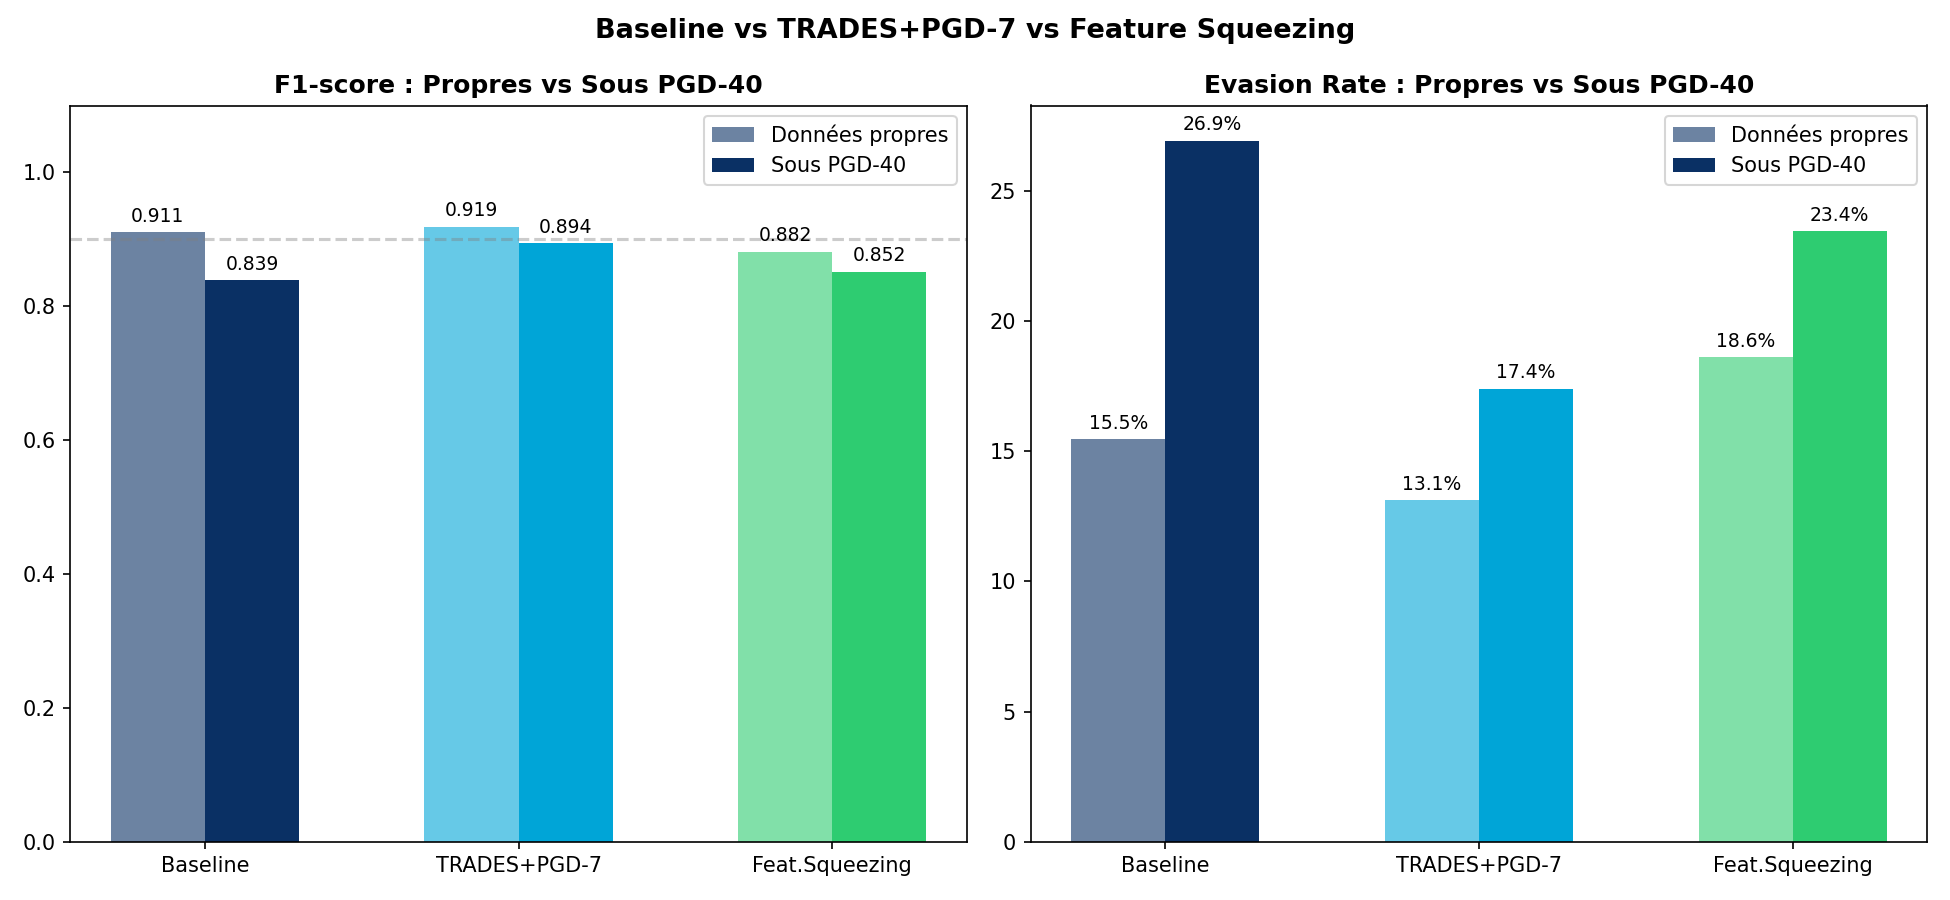
\includegraphics[width=0.88\textwidth,height=6.5cm,keepaspectratio]{../results/trades_comparison.png}
\end{frame}

%% ============================================================
%% SLIDE 11 — CONCLUSION & PERSPECTIVES
%% ============================================================
\begin{frame}{Conclusion \& Perspectives}
\begin{columns}[T]
\column{0.50\textwidth}
\begin{block}{Bilan des r\'esultats}
\footnotesize
\begin{tabular}{lr}
\toprule
\textbf{Configuration} & \textbf{Evasion PGD-40} \\
\midrule
Baseline               & 28.2\% \\
Adv. Training          & \alert{36--41\%} \\
Feature Squeezing      & 24.5\% \\
TRADES + PGD-7         & 17.4\% \\
\rowcolor{inptblue!30}
\textbf{TRADES + FS}   & \textbf{10.7\%} \\
\bottomrule
\end{tabular}
\end{block}

\column{0.47\textwidth}
\begin{exampleblock}{Perspectives}
Avec plus de temps et de ressources :
\begin{itemize}\setlength\itemsep{3pt}
    \item Seuil 0.40 sur TRADES seul $\Rightarrow$ \textbf{14.7\%}
    \item TRADES + FS + seuil 0.45 $\Rightarrow$ \textbf{7.8\%}
    \item AutoAttack (\'evaluation plus rigoureuse)
    \item Randomized Smoothing (robustesse certifi\'ee)
\end{itemize}
\end{exampleblock}
\end{columns}
\end{frame}

%% ============================================================
%% SLIDE 12 — MERCI
%% ============================================================
\begin{frame}[plain]
\begin{tikzpicture}[remember picture, overlay]
  \fill[inptblue] (current page.south west) rectangle (current page.north east);
  \fill[inptcyan] ([yshift=0.6cm]current page.south west)
                  rectangle ([yshift=0.9cm]current page.south east);
\end{tikzpicture}
\begin{center}
\vspace{2.5cm}
{\LARGE\bfseries\color{white} Merci pour votre attention}\\[0.8em]
{\large\color{inptcyan} Questions ?}\\[2em]
{\footnotesize\color{white!80}
FGSM : Goodfellow et al., ICLR 2015 \quad
PGD : Madry et al., ICLR 2018 \quad
TRADES : Zhang et al., ICML 2019}
\end{center}
\end{frame}

\end{document}
